\subsubsection{Formiranje evidencije o zaposlenima}
\label{subsubsec:vozni park}
\begin{itemize}
  \item \textbf{Kratak opis}: Nadležni za zaposlene ima mogućnost da vodi evidenciju kadrova zaposlenih u auto školi 
  (instruktora, predavača, računovođa, administrativnih radnika). Vodi računa o rasporedu rada, radnom vremenu i slobodnim danima zaposlenih.

  \item \textbf{Učesnici}:
    \begin{itemize}
    \item Nadležni za zaposlene - korisnik sistema koji vodi evidenciju o zaposlenima.
    \end{itemize}
  \item \textbf{Preduslovi}:
    \begin{itemize}
    \item  Nadležni za zaposlene je uspešno ulogovan na sistem auto škole.
    \item  Sistem je u funkciji.
    \item  Nadležni za zaposlene ima pristup internetu.
    \end{itemize}
  \item \textbf{Postuslovi}:
      \begin{itemize}
      \item  Nadležni za zaposlene je ažurirao evidenciju o zaposlenim kadrovima u auto školi.
      \item  Nadležni za zaposlene je ažurirao evidenciju o rasporedu rada zaposlenih.
      \end{itemize}
  \item \textbf{Osnovni tok}:
      \begin{enumerate}
        \item Nadležni za zaposlene otvara stranicu za uvid u spisak zaposlenih radnika.
        \item Sistem prikazuje trenutno zaposlene kao i njihov raspored rada za tekuću nedelju.
        \item Nadležni pritiska dugme "Izmeni" na stranici.
        \item Sistem omogućava organizatoru da izmeni podatke u tabeli.
        \item Nadležni menja radno vreme nekom zaposlenom po potrebi.
        \item Nadležni potvrđuje izmene.
        \item Sistem evidentira izmene.
        \item Sistem šalje mejl o izmenama zaposlenima ako je došlo do novog rasporeda rada za narednu nedelju.
      \end{enumerate}

  \item \textbf{Alternativni tokovi}:
      \begin{itemize}
        \item A1. \textbf{Neuspela validacija.}
        Ukoliko u koraku 5 nadležni u formu o izmenama unese nevalidne podatke polja formulara koja su neispravna će biti crvena.
        Nakon što nadležni ažurira podatke nastavlja se čuvanje izmena. Proces se nastavlja u koraku 6.
      \end{itemize}

      
  \item \textbf{Specijalni zahtevi}:
      \begin{itemize}
        \item Podaci o zaposlenom : ime, prezime, jmbg, broj telefona, raspored rada.
      \end{itemize}
\end{itemize}

\begin{figure}[H]
  \begin{center}
      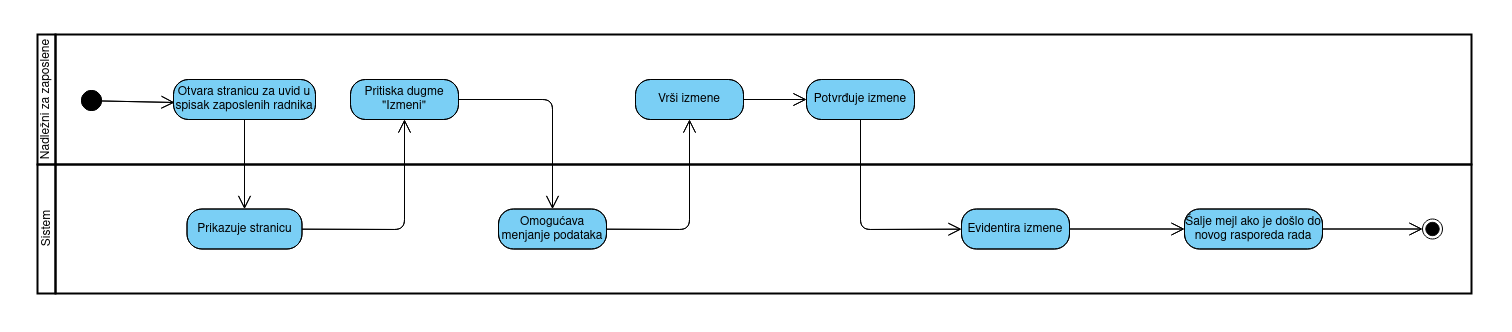
\includegraphics[width=140mm, height=70mm]{Diagrams/evidencija_zaposlenih.png}
  \end{center}
  \caption {Dijagram aktivnosti - Formiranje evidencije o zaposlenima}
  \label{activity_evidencija_zaposlenih}

\end{figure}
